\documentclass[14pt]{extbook}
\usepackage{multicol, enumerate, enumitem, hyperref, color, soul, setspace, parskip, fancyhdr} %General Packages
\usepackage{amssymb, amsthm, amsmath, latexsym, units, mathtools} %Math Packages
\everymath{\displaystyle} %All math in Display Style
% Packages with additional options
\usepackage[headsep=0.5cm,headheight=12pt, left=1 in,right= 1 in,top= 1 in,bottom= 1 in]{geometry}
\usepackage[usenames,dvipsnames]{xcolor}
\usepackage{dashrule}  % Package to use the command below to create lines between items
\newcommand{\litem}[1]{\item#1\hspace*{-1cm}\rule{\textwidth}{0.4pt}}
\pagestyle{fancy}
\lhead{Progress Quiz 6}
\chead{}
\rhead{Version ALL}
\lfoot{4563-7456}
\cfoot{}
\rfoot{Summer C 2021}
\begin{document}

\begin{enumerate}
\litem{
Construct the lowest-degree polynomial given the zeros below. Then, choose the intervals that contain the coefficients of the polynomial in the form $x^3+bx^2+cx+d$.\[ -3 - 2 i \text{ and } -3 \]\begin{enumerate}[label=\Alph*.]
\item \( b \in [-5, 3], c \in [5.4, 6.45], \text{ and } d \in [7.9, 9.4] \)
\item \( b \in [-5, 3], c \in [4.58, 5.53], \text{ and } d \in [1.9, 7.1] \)
\item \( b \in [2, 13], c \in [30.15, 31.6], \text{ and } d \in [38.1, 39.8] \)
\item \( b \in [-17, -6], c \in [30.15, 31.6], \text{ and } d \in [-42, -38.7] \)
\item \( \text{None of the above.} \)

\end{enumerate} }
\litem{
Which of the following equations \textit{could} be of the graph presented below?
\begin{center}
    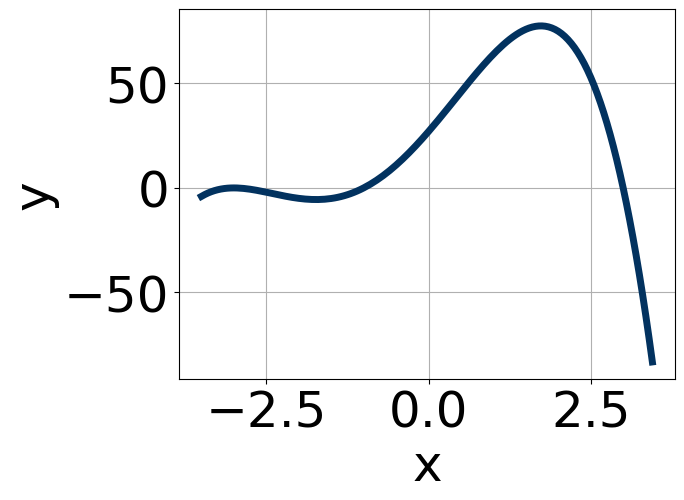
\includegraphics[width=0.5\textwidth]{../Figures/polyGraphToFunctionA.png}
\end{center}
\begin{enumerate}[label=\Alph*.]
\item \( -15(x + 3)^{10} (x - 3)^{7} (x + 1)^{11} \)
\item \( -9(x + 3)^{11} (x - 3)^{8} (x + 1)^{9} \)
\item \( -7(x + 3)^{10} (x - 3)^{6} (x + 1)^{7} \)
\item \( 5(x + 3)^{10} (x - 3)^{5} (x + 1)^{4} \)
\item \( 7(x + 3)^{6} (x - 3)^{5} (x + 1)^{5} \)

\end{enumerate} }
\litem{
Which of the following equations \textit{could} be of the graph presented below?
\begin{center}
    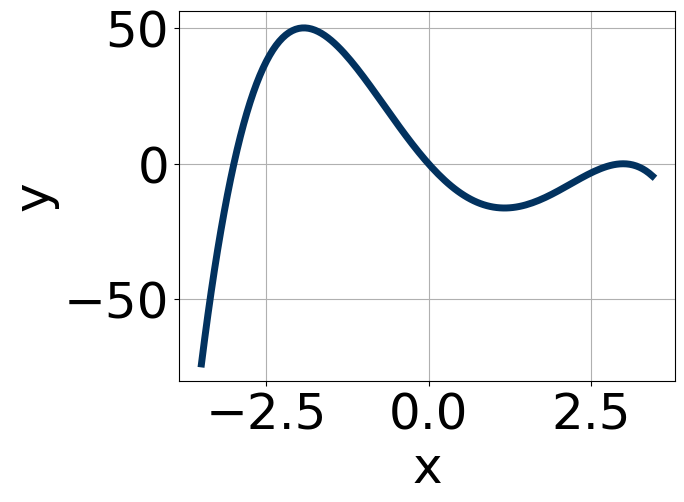
\includegraphics[width=0.5\textwidth]{../Figures/polyGraphToFunctionCopyA.png}
\end{center}
\begin{enumerate}[label=\Alph*.]
\item \( 10x^{7} (x - 3)^{4} (x + 3)^{10} \)
\item \( 15x^{11} (x - 3)^{6} (x + 3)^{5} \)
\item \( -20x^{6} (x - 3)^{9} (x + 3)^{7} \)
\item \( -7x^{7} (x - 3)^{8} (x + 3)^{5} \)
\item \( -18x^{4} (x - 3)^{4} (x + 3)^{5} \)

\end{enumerate} }
\litem{
Describe the zero behavior of the zero $x = 4$ of the polynomial below.\[ f(x) = 2(x + 6)^{8}(x - 6)^{4}(x - 4)^{10}(x + 4)^{7} \]\begin{enumerate}[label=\Alph*.]
\begin{multicols}{2}\item 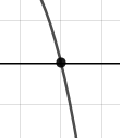
\includegraphics[width = 0.3\textwidth]{../Figures/polyZeroBehaviorCopyAA.png}\item 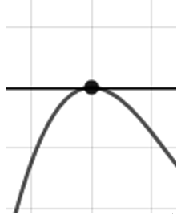
\includegraphics[width = 0.3\textwidth]{../Figures/polyZeroBehaviorCopyBA.png}\item 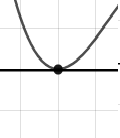
\includegraphics[width = 0.3\textwidth]{../Figures/polyZeroBehaviorCopyCA.png}\item 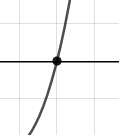
\includegraphics[width = 0.3\textwidth]{../Figures/polyZeroBehaviorCopyDA.png}\end{multicols}\item None of the above.
\end{enumerate} }
\litem{
Construct the lowest-degree polynomial given the zeros below. Then, choose the intervals that contain the coefficients of the polynomial in the form $x^3+bx^2+cx+d$.\[ 2 + 3 i \text{ and } 3 \]\begin{enumerate}[label=\Alph*.]
\item \( b \in [4, 11], c \in [21.54, 25.63], \text{ and } d \in [33, 43] \)
\item \( b \in [-3, 5], c \in [-5.17, -2.87], \text{ and } d \in [0, 7] \)
\item \( b \in [-3, 5], c \in [-6.83, -5.89], \text{ and } d \in [9, 10] \)
\item \( b \in [-9, -4], c \in [21.54, 25.63], \text{ and } d \in [-46, -38] \)
\item \( \text{None of the above.} \)

\end{enumerate} }
\litem{
Construct the lowest-degree polynomial given the zeros below. Then, choose the intervals that contain the coefficients of the polynomial in the form $ax^3+bx^2+cx+d$.\[ \frac{3}{5}, \frac{-1}{3}, \text{ and } \frac{-1}{2} \]\begin{enumerate}[label=\Alph*.]
\item \( a \in [30, 39], b \in [-13, -1], c \in [-13, -6], \text{ and } d \in [-1, 7] \)
\item \( a \in [30, 39], b \in [40, 44], c \in [18, 24], \text{ and } d \in [-1, 7] \)
\item \( a \in [30, 39], b \in [22, 27], c \in [-2, 0], \text{ and } d \in [-3, -2] \)
\item \( a \in [30, 39], b \in [7, 13], c \in [-13, -6], \text{ and } d \in [-1, 7] \)
\item \( a \in [30, 39], b \in [7, 13], c \in [-13, -6], \text{ and } d \in [-3, -2] \)

\end{enumerate} }
\litem{
Describe the end behavior of the polynomial below.\[ f(x) = -7(x - 9)^{5}(x + 9)^{8}(x + 4)^{5}(x - 4)^{7} \]\begin{enumerate}[label=\Alph*.]
\begin{multicols}{2}\item 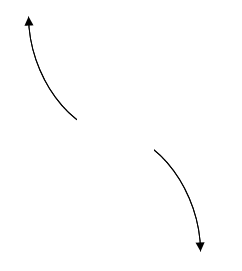
\includegraphics[width = 0.3\textwidth]{../Figures/polyEndBehaviorAA.png}\item 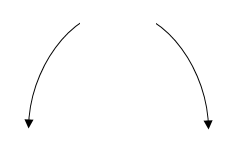
\includegraphics[width = 0.3\textwidth]{../Figures/polyEndBehaviorBA.png}\item 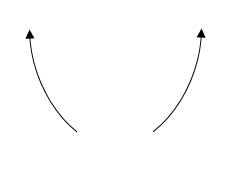
\includegraphics[width = 0.3\textwidth]{../Figures/polyEndBehaviorCA.png}\item 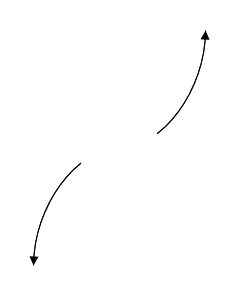
\includegraphics[width = 0.3\textwidth]{../Figures/polyEndBehaviorDA.png}\end{multicols}\item None of the above.
\end{enumerate} }
\litem{
Construct the lowest-degree polynomial given the zeros below. Then, choose the intervals that contain the coefficients of the polynomial in the form $ax^3+bx^2+cx+d$.\[ \frac{-6}{5}, \frac{3}{5}, \text{ and } \frac{7}{2} \]\begin{enumerate}[label=\Alph*.]
\item \( a \in [48, 54], b \in [-154, -139], c \in [-141, -135], \text{ and } d \in [-128, -118] \)
\item \( a \in [48, 54], b \in [-206, -201], c \in [67, 73], \text{ and } d \in [125, 132] \)
\item \( a \in [48, 54], b \in [-267, -261], c \in [350, 357], \text{ and } d \in [-128, -118] \)
\item \( a \in [48, 54], b \in [142, 152], c \in [-141, -135], \text{ and } d \in [-128, -118] \)
\item \( a \in [48, 54], b \in [-154, -139], c \in [-141, -135], \text{ and } d \in [125, 132] \)

\end{enumerate} }
\litem{
Describe the zero behavior of the zero $x = 5$ of the polynomial below.\[ f(x) = -7(x - 3)^{6}(x + 3)^{3}(x - 5)^{10}(x + 5)^{7} \]\begin{enumerate}[label=\Alph*.]
\begin{multicols}{2}\item 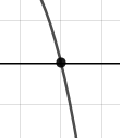
\includegraphics[width = 0.3\textwidth]{../Figures/polyZeroBehaviorAA.png}\item 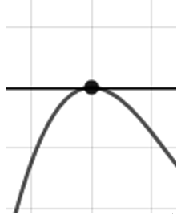
\includegraphics[width = 0.3\textwidth]{../Figures/polyZeroBehaviorBA.png}\item 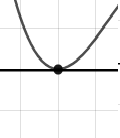
\includegraphics[width = 0.3\textwidth]{../Figures/polyZeroBehaviorCA.png}\item 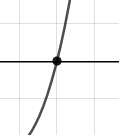
\includegraphics[width = 0.3\textwidth]{../Figures/polyZeroBehaviorDA.png}\end{multicols}\item None of the above.
\end{enumerate} }
\litem{
Describe the end behavior of the polynomial below.\[ f(x) = -8(x + 3)^{4}(x - 3)^{5}(x + 7)^{3}(x - 7)^{5} \]\begin{enumerate}[label=\Alph*.]
\begin{multicols}{2}\item 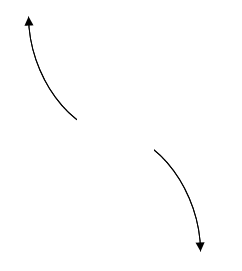
\includegraphics[width = 0.3\textwidth]{../Figures/polyEndBehaviorCopyAA.png}\item 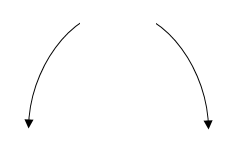
\includegraphics[width = 0.3\textwidth]{../Figures/polyEndBehaviorCopyBA.png}\item 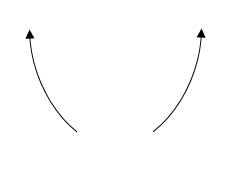
\includegraphics[width = 0.3\textwidth]{../Figures/polyEndBehaviorCopyCA.png}\item 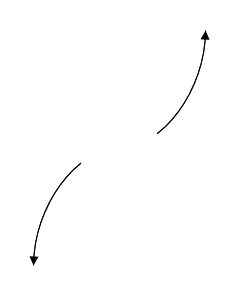
\includegraphics[width = 0.3\textwidth]{../Figures/polyEndBehaviorCopyDA.png}\end{multicols}\item None of the above.
\end{enumerate} }
\litem{
Construct the lowest-degree polynomial given the zeros below. Then, choose the intervals that contain the coefficients of the polynomial in the form $x^3+bx^2+cx+d$.\[ -5 + 5 i \text{ and } 3 \]\begin{enumerate}[label=\Alph*.]
\item \( b \in [-11, -3], c \in [16, 22], \text{ and } d \in [145, 151] \)
\item \( b \in [1, 6], c \in [-1, 7], \text{ and } d \in [-18, -13] \)
\item \( b \in [2, 12], c \in [16, 22], \text{ and } d \in [-156, -141] \)
\item \( b \in [1, 6], c \in [-9, 1], \text{ and } d \in [13, 20] \)
\item \( \text{None of the above.} \)

\end{enumerate} }
\litem{
Which of the following equations \textit{could} be of the graph presented below?
\begin{center}
    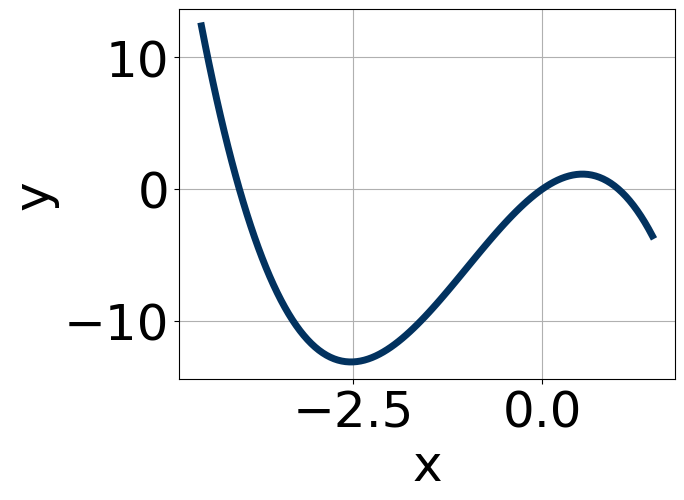
\includegraphics[width=0.5\textwidth]{../Figures/polyGraphToFunctionB.png}
\end{center}
\begin{enumerate}[label=\Alph*.]
\item \( -9x^{5} (x - 1)^{9} (x + 4)^{9} \)
\item \( 17x^{11} (x - 1)^{9} (x + 4)^{9} \)
\item \( 6x^{5} (x - 1)^{8} (x + 4)^{9} \)
\item \( -7x^{7} (x - 1)^{8} (x + 4)^{4} \)
\item \( -17x^{7} (x - 1)^{10} (x + 4)^{9} \)

\end{enumerate} }
\litem{
Which of the following equations \textit{could} be of the graph presented below?
\begin{center}
    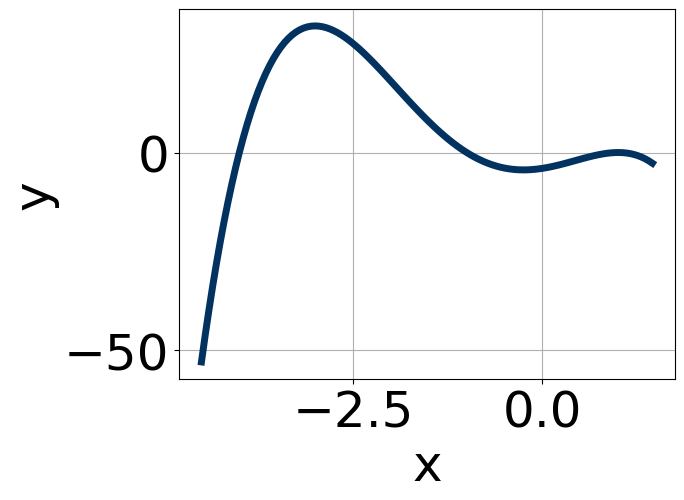
\includegraphics[width=0.5\textwidth]{../Figures/polyGraphToFunctionCopyB.png}
\end{center}
\begin{enumerate}[label=\Alph*.]
\item \( -17(x - 1)^{4} (x + 4)^{8} (x + 1)^{9} \)
\item \( 20(x - 1)^{10} (x + 4)^{7} (x + 1)^{4} \)
\item \( 2(x - 1)^{10} (x + 4)^{9} (x + 1)^{9} \)
\item \( -6(x - 1)^{7} (x + 4)^{8} (x + 1)^{11} \)
\item \( -4(x - 1)^{10} (x + 4)^{7} (x + 1)^{9} \)

\end{enumerate} }
\litem{
Describe the zero behavior of the zero $x = -6$ of the polynomial below.\[ f(x) = -4(x - 8)^{6}(x + 8)^{2}(x + 6)^{9}(x - 6)^{6} \]\begin{enumerate}[label=\Alph*.]
\begin{multicols}{2}\item 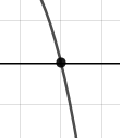
\includegraphics[width = 0.3\textwidth]{../Figures/polyZeroBehaviorCopyAB.png}\item 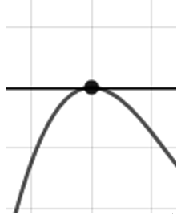
\includegraphics[width = 0.3\textwidth]{../Figures/polyZeroBehaviorCopyBB.png}\item 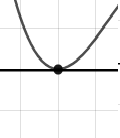
\includegraphics[width = 0.3\textwidth]{../Figures/polyZeroBehaviorCopyCB.png}\item 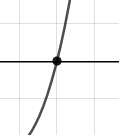
\includegraphics[width = 0.3\textwidth]{../Figures/polyZeroBehaviorCopyDB.png}\end{multicols}\item None of the above.
\end{enumerate} }
\litem{
Construct the lowest-degree polynomial given the zeros below. Then, choose the intervals that contain the coefficients of the polynomial in the form $x^3+bx^2+cx+d$.\[ -4 - 2 i \text{ and } -2 \]\begin{enumerate}[label=\Alph*.]
\item \( b \in [8, 13], c \in [34.2, 37], \text{ and } d \in [40, 42] \)
\item \( b \in [-4, 6], c \in [4.5, 8.2], \text{ and } d \in [6, 9] \)
\item \( b \in [-4, 6], c \in [3, 4.3], \text{ and } d \in [2, 5] \)
\item \( b \in [-14, -8], c \in [34.2, 37], \text{ and } d \in [-40, -32] \)
\item \( \text{None of the above.} \)

\end{enumerate} }
\litem{
Construct the lowest-degree polynomial given the zeros below. Then, choose the intervals that contain the coefficients of the polynomial in the form $ax^3+bx^2+cx+d$.\[ \frac{-7}{5}, \frac{5}{2}, \text{ and } \frac{-1}{4} \]\begin{enumerate}[label=\Alph*.]
\item \( a \in [35, 41], b \in [48, 58], c \in [-131, -125], \text{ and } d \in [-42, -32] \)
\item \( a \in [35, 41], b \in [-36, -27], c \in [-158, -150], \text{ and } d \in [33, 37] \)
\item \( a \in [35, 41], b \in [-148, -145], c \in [95, 106], \text{ and } d \in [33, 37] \)
\item \( a \in [35, 41], b \in [-36, -27], c \in [-158, -150], \text{ and } d \in [-42, -32] \)
\item \( a \in [35, 41], b \in [32, 40], c \in [-158, -150], \text{ and } d \in [33, 37] \)

\end{enumerate} }
\litem{
Describe the end behavior of the polynomial below.\[ f(x) = 8(x - 4)^{4}(x + 4)^{9}(x + 8)^{4}(x - 8)^{5} \]\begin{enumerate}[label=\Alph*.]
\begin{multicols}{2}\item 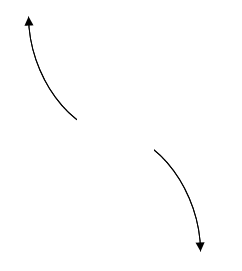
\includegraphics[width = 0.3\textwidth]{../Figures/polyEndBehaviorAB.png}\item 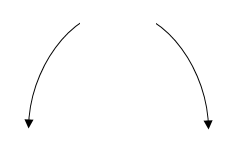
\includegraphics[width = 0.3\textwidth]{../Figures/polyEndBehaviorBB.png}\item 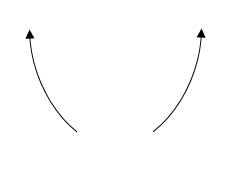
\includegraphics[width = 0.3\textwidth]{../Figures/polyEndBehaviorCB.png}\item 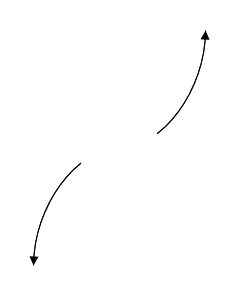
\includegraphics[width = 0.3\textwidth]{../Figures/polyEndBehaviorDB.png}\end{multicols}\item None of the above.
\end{enumerate} }
\litem{
Construct the lowest-degree polynomial given the zeros below. Then, choose the intervals that contain the coefficients of the polynomial in the form $ax^3+bx^2+cx+d$.\[ \frac{1}{2}, \frac{7}{4}, \text{ and } 4 \]\begin{enumerate}[label=\Alph*.]
\item \( a \in [7, 12], b \in [-23, -12], c \in [-71, -59], \text{ and } d \in [-32, -21] \)
\item \( a \in [7, 12], b \in [-51, -44], c \in [77, 82], \text{ and } d \in [-32, -21] \)
\item \( a \in [7, 12], b \in [49, 55], c \in [77, 82], \text{ and } d \in [28, 30] \)
\item \( a \in [7, 12], b \in [-51, -44], c \in [77, 82], \text{ and } d \in [28, 30] \)
\item \( a \in [7, 12], b \in [-44, -34], c \in [31, 43], \text{ and } d \in [28, 30] \)

\end{enumerate} }
\litem{
Describe the zero behavior of the zero $x = 2$ of the polynomial below.\[ f(x) = -4(x - 2)^{5}(x + 2)^{10}(x - 3)^{6}(x + 3)^{10} \]\begin{enumerate}[label=\Alph*.]
\begin{multicols}{2}\item 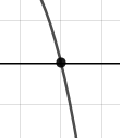
\includegraphics[width = 0.3\textwidth]{../Figures/polyZeroBehaviorAB.png}\item 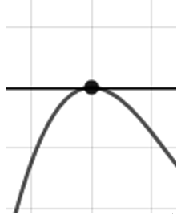
\includegraphics[width = 0.3\textwidth]{../Figures/polyZeroBehaviorBB.png}\item 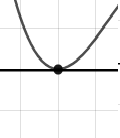
\includegraphics[width = 0.3\textwidth]{../Figures/polyZeroBehaviorCB.png}\item 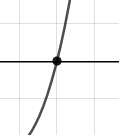
\includegraphics[width = 0.3\textwidth]{../Figures/polyZeroBehaviorDB.png}\end{multicols}\item None of the above.
\end{enumerate} }
\litem{
Describe the end behavior of the polynomial below.\[ f(x) = 2(x + 5)^{3}(x - 5)^{6}(x + 3)^{3}(x - 3)^{5} \]\begin{enumerate}[label=\Alph*.]
\begin{multicols}{2}\item 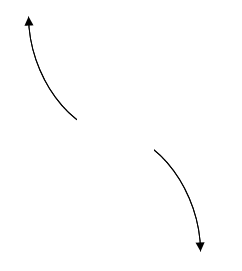
\includegraphics[width = 0.3\textwidth]{../Figures/polyEndBehaviorCopyAB.png}\item 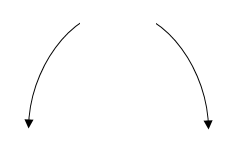
\includegraphics[width = 0.3\textwidth]{../Figures/polyEndBehaviorCopyBB.png}\item 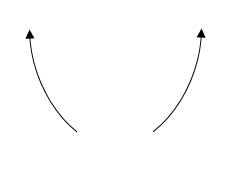
\includegraphics[width = 0.3\textwidth]{../Figures/polyEndBehaviorCopyCB.png}\item 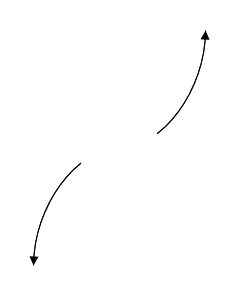
\includegraphics[width = 0.3\textwidth]{../Figures/polyEndBehaviorCopyDB.png}\end{multicols}\item None of the above.
\end{enumerate} }
\litem{
Construct the lowest-degree polynomial given the zeros below. Then, choose the intervals that contain the coefficients of the polynomial in the form $x^3+bx^2+cx+d$.\[ -2 - 5 i \text{ and } 3 \]\begin{enumerate}[label=\Alph*.]
\item \( b \in [-0.9, 3.8], c \in [16, 20.1], \text{ and } d \in [-91, -82] \)
\item \( b \in [-1.5, 0.8], c \in [16, 20.1], \text{ and } d \in [84, 91] \)
\item \( b \in [-0.9, 3.8], c \in [-3.2, -0.5], \text{ and } d \in [-6, -1] \)
\item \( b \in [-0.9, 3.8], c \in [0.2, 7.4], \text{ and } d \in [-15, -11] \)
\item \( \text{None of the above.} \)

\end{enumerate} }
\litem{
Which of the following equations \textit{could} be of the graph presented below?
\begin{center}
    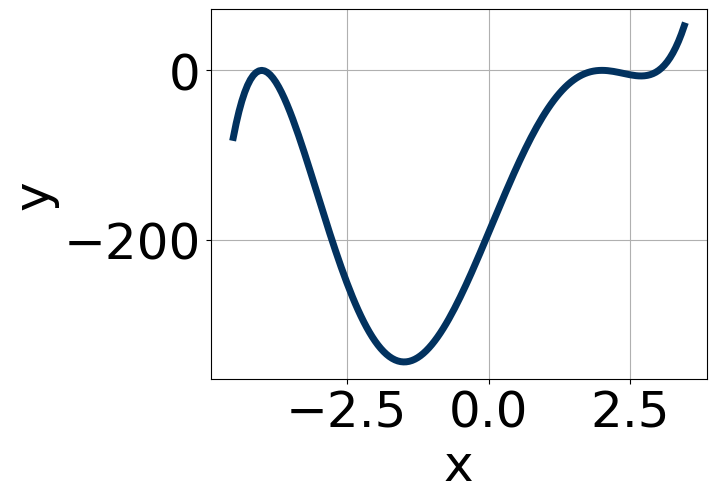
\includegraphics[width=0.5\textwidth]{../Figures/polyGraphToFunctionC.png}
\end{center}
\begin{enumerate}[label=\Alph*.]
\item \( 13(x + 4)^{6} (x - 2)^{5} (x - 3)^{9} \)
\item \( -18(x + 4)^{4} (x - 2)^{10} (x - 3)^{6} \)
\item \( 8(x + 4)^{6} (x - 2)^{8} (x - 3)^{9} \)
\item \( 3(x + 4)^{8} (x - 2)^{9} (x - 3)^{4} \)
\item \( -8(x + 4)^{4} (x - 2)^{8} (x - 3)^{5} \)

\end{enumerate} }
\litem{
Which of the following equations \textit{could} be of the graph presented below?
\begin{center}
    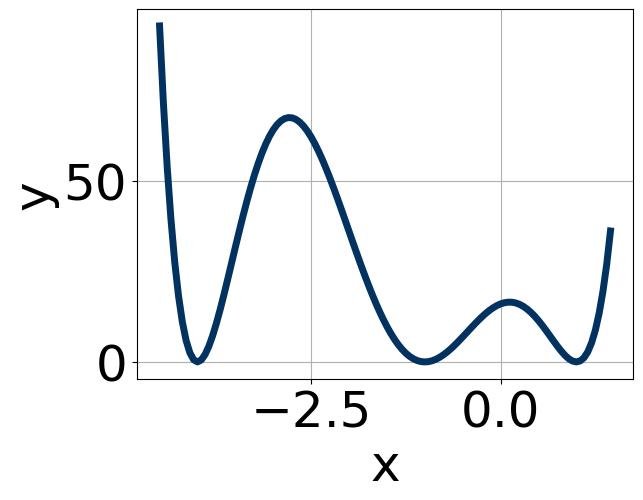
\includegraphics[width=0.5\textwidth]{../Figures/polyGraphToFunctionCopyC.png}
\end{center}
\begin{enumerate}[label=\Alph*.]
\item \( -18(x + 4)^{10} (x + 1)^{4} (x - 1)^{8} \)
\item \( 20(x + 4)^{8} (x + 1)^{5} (x - 1)^{7} \)
\item \( 18(x + 4)^{6} (x + 1)^{4} (x - 1)^{8} \)
\item \( -4(x + 4)^{10} (x + 1)^{10} (x - 1)^{7} \)
\item \( 6(x + 4)^{8} (x + 1)^{4} (x - 1)^{7} \)

\end{enumerate} }
\litem{
Describe the zero behavior of the zero $x = 6$ of the polynomial below.\[ f(x) = -3(x + 4)^{8}(x - 4)^{5}(x + 6)^{6}(x - 6)^{5} \]\begin{enumerate}[label=\Alph*.]
\begin{multicols}{2}\item 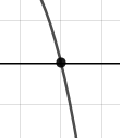
\includegraphics[width = 0.3\textwidth]{../Figures/polyZeroBehaviorCopyAC.png}\item 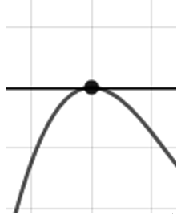
\includegraphics[width = 0.3\textwidth]{../Figures/polyZeroBehaviorCopyBC.png}\item 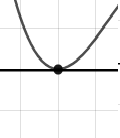
\includegraphics[width = 0.3\textwidth]{../Figures/polyZeroBehaviorCopyCC.png}\item 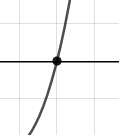
\includegraphics[width = 0.3\textwidth]{../Figures/polyZeroBehaviorCopyDC.png}\end{multicols}\item None of the above.
\end{enumerate} }
\litem{
Construct the lowest-degree polynomial given the zeros below. Then, choose the intervals that contain the coefficients of the polynomial in the form $x^3+bx^2+cx+d$.\[ -2 + 5 i \text{ and } 1 \]\begin{enumerate}[label=\Alph*.]
\item \( b \in [2.3, 3.6], c \in [24, 32], \text{ and } d \in [-30, -20] \)
\item \( b \in [-1.2, 1.7], c \in [-10, -3], \text{ and } d \in [0, 12] \)
\item \( b \in [-1.2, 1.7], c \in [-1, 13], \text{ and } d \in [-5, 0] \)
\item \( b \in [-5.5, -1.7], c \in [24, 32], \text{ and } d \in [23, 32] \)
\item \( \text{None of the above.} \)

\end{enumerate} }
\litem{
Construct the lowest-degree polynomial given the zeros below. Then, choose the intervals that contain the coefficients of the polynomial in the form $ax^3+bx^2+cx+d$.\[ 2, \frac{1}{5}, \text{ and } \frac{-1}{4} \]\begin{enumerate}[label=\Alph*.]
\item \( a \in [17, 29], b \in [-39.3, -36.6], c \in [-5.1, -0.4], \text{ and } d \in [-4, 0] \)
\item \( a \in [17, 29], b \in [47.6, 51.5], c \in [18.7, 20.3], \text{ and } d \in [2, 8] \)
\item \( a \in [17, 29], b \in [-39.3, -36.6], c \in [-5.1, -0.4], \text{ and } d \in [2, 8] \)
\item \( a \in [17, 29], b \in [33.4, 40.5], c \in [-5.1, -0.4], \text{ and } d \in [-4, 0] \)
\item \( a \in [17, 29], b \in [39.7, 41.9], c \in [-2, 2.2], \text{ and } d \in [-4, 0] \)

\end{enumerate} }
\litem{
Describe the end behavior of the polynomial below.\[ f(x) = 5(x - 5)^{4}(x + 5)^{5}(x - 6)^{5}(x + 6)^{6} \]\begin{enumerate}[label=\Alph*.]
\begin{multicols}{2}\item 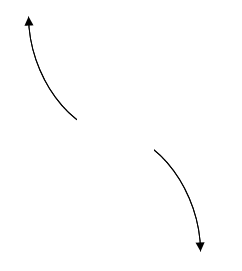
\includegraphics[width = 0.3\textwidth]{../Figures/polyEndBehaviorAC.png}\item 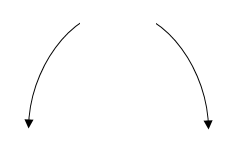
\includegraphics[width = 0.3\textwidth]{../Figures/polyEndBehaviorBC.png}\item 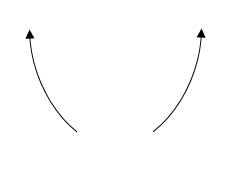
\includegraphics[width = 0.3\textwidth]{../Figures/polyEndBehaviorCC.png}\item 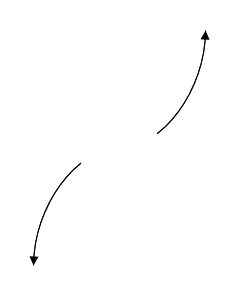
\includegraphics[width = 0.3\textwidth]{../Figures/polyEndBehaviorDC.png}\end{multicols}\item None of the above.
\end{enumerate} }
\litem{
Construct the lowest-degree polynomial given the zeros below. Then, choose the intervals that contain the coefficients of the polynomial in the form $ax^3+bx^2+cx+d$.\[ -5, \frac{-2}{3}, \text{ and } \frac{-7}{5} \]\begin{enumerate}[label=\Alph*.]
\item \( a \in [12, 16], b \in [103, 110], c \in [161, 178], \text{ and } d \in [-74, -62] \)
\item \( a \in [12, 16], b \in [-72, -57], c \in [-75, -65], \text{ and } d \in [68, 74] \)
\item \( a \in [12, 16], b \in [-45, -43], c \in [-142, -136], \text{ and } d \in [-74, -62] \)
\item \( a \in [12, 16], b \in [-113, -105], c \in [161, 178], \text{ and } d \in [-74, -62] \)
\item \( a \in [12, 16], b \in [103, 110], c \in [161, 178], \text{ and } d \in [68, 74] \)

\end{enumerate} }
\litem{
Describe the zero behavior of the zero $x = -9$ of the polynomial below.\[ f(x) = -9(x - 9)^{4}(x + 9)^{5}(x + 3)^{9}(x - 3)^{10} \]\begin{enumerate}[label=\Alph*.]
\begin{multicols}{2}\item 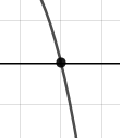
\includegraphics[width = 0.3\textwidth]{../Figures/polyZeroBehaviorAC.png}\item 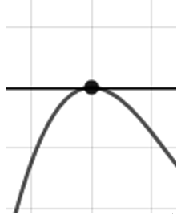
\includegraphics[width = 0.3\textwidth]{../Figures/polyZeroBehaviorBC.png}\item 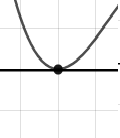
\includegraphics[width = 0.3\textwidth]{../Figures/polyZeroBehaviorCC.png}\item 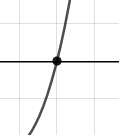
\includegraphics[width = 0.3\textwidth]{../Figures/polyZeroBehaviorDC.png}\end{multicols}\item None of the above.
\end{enumerate} }
\litem{
Describe the end behavior of the polynomial below.\[ f(x) = 5(x - 5)^{5}(x + 5)^{10}(x - 8)^{5}(x + 8)^{7} \]\begin{enumerate}[label=\Alph*.]
\begin{multicols}{2}\item \includegraphics[width = 0.3\textwidth]{../Figures/polyEndBehaviorCopyAC.png}\item \includegraphics[width = 0.3\textwidth]{../Figures/polyEndBehaviorCopyBC.png}\item \includegraphics[width = 0.3\textwidth]{../Figures/polyEndBehaviorCopyCC.png}\item \includegraphics[width = 0.3\textwidth]{../Figures/polyEndBehaviorCopyDC.png}\end{multicols}\item None of the above.
\end{enumerate} }
\end{enumerate}

\end{document}